\section{METHODOLOGY}
\label{sec:approach}

\begin{figure}[t]
   \centering
   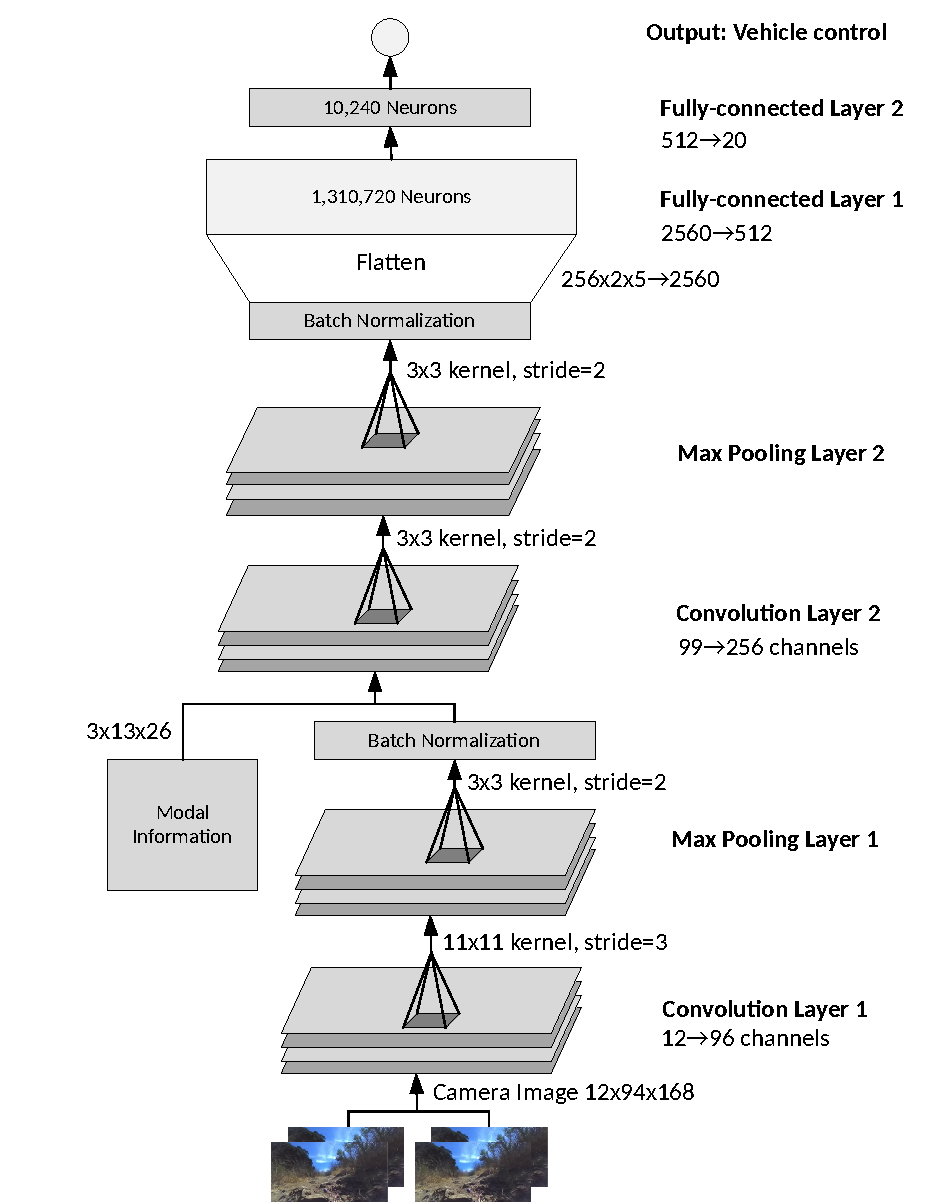
\includegraphics[width=\columnwidth,trim=0 0 20 0,clip]{paper/content/images/z2color}
   \caption{MultiNet Z2Color Network Architecture with Modal Insertion}
   \label{fig:squeeze}
\end{figure}
% Each network is trained with the Adadelta Optimizer \cite{DBLP:journals/corr/abs-1212-5701} and uses MSE Loss to compare ground truth and network output.

\subsection{Network Architecture}
For inference, we employ an NVIDIA Jetson TX1 system, and run a custom network we call Z2Color at a 20 Hz frequency. The network consists of two convolutional layers, followed by two fully connected layers shown in (\Cref{fig:squeeze}).

Max pooling and batch normalization were done after each convolutional layer. Max pooling allowed us to efficiently reduce dimensionality and batch normalization prevented internal covariate shift \cite{ioffe2015batch}. The stride and kernel sizes were found empirically through numerous cycles of training and on-road evaluation.
The convolutional layers were designed to act as feature extraction layers whereas the final fully connected layers act as a steering controller. However, the network was trained in an end-to-end manner so we did not isolate different forms of processing to specific sections of the network.

The network is compact, with no more than 1.7 million parameters, taking approximately 6.5 MB for each model, allowing for Field Programmable Gate Array (FPGA) or Application-Specific Integrated Circuit (ASIC) deployment. Iandola states ``FPGAs often have less than 10MB of on chip memory and no off-chip memory or storage. For inference, a sufficiently small model could be stored directly on the FPGA instead of being bottlenecked by memory bandwidth." \cite{DBLP:journals/corr/IandolaMAHDK16}

%In inference mode, small models have been shown to be able to be stored on FPGAs to avoid memory bandwith bottlenecks \cite{qiu2016going}. It is standard for FPGAs to contain fewer than 10 MB of block memory on the chip and no expandable memory \footnote{The popular Xilinx Vertex-7 FPGA has a maximum Total Block Ram of 8.5 MB of on chip memory with no expandable memory off-chip.} Similarly, for deployment of DNNs on ASICs, a small model is necessary to be stored directly on chip \cite{DBLP:journals/corr/IandolaMAHDK16}.

While a single MultiNet Z2Color network could fit on such a platform, multiple MTL Z2Color networks trained for just two behavioral modalities would result in a 13 MB model incapable of running directly on a 10 MB FPGA. For these reasons, as the number of modalities increases multiple distinct networks become increasingly impractical for deployment whereas a MultiNet Z2Color network allows for deployment on faster platforms with smaller network sizes.

% We wanted to choose a compact but powerful DNN, that could be run at 20 Hz or above on the NVIDIA TX1 board. The network that fit these criteria for us was SqueezeNet \cite{DBLP:journals/corr/IandolaMAHDK16}. It has been shown to match the performance of AlexNet with 500x fewer parameters in the network. It has also been shown to perform well in Autonomous Driving Tasks \cite{tusharsfuturepaper}. In order to use this network we need to make some simple modifications to the input and output of our network.

\subsection{Modal Information}

When collecting data from the cars, along with motor, steering, and image data, we also store the behavioral mode in which the car is being operated. We have trained networks with and without the insertion of the behavioral information and when added, networks more distinctly exhibit individual modal behaviors.

A network without this modal information could potentially learn multiple behavioral modes distinctly, but it would take a great amount of careful training for the filters to separate for each behavioral modality. By adding the logical modal switch in the processing stream, it becomes easier for the network to create independent filters for each behavioral mode.

The behavioral information is inserted as a three channel binary tensor, where each channel represents a different behavioral modality. In order to concatenate with the image going through the convolutional network, the behavioral information is replicated in the spatial dimensions to form a binary tensor of size 3x13x26. The behavioral mode information insertion point in the network was chosen to be after the first convolutional layer in Z2Color (\Cref{fig:squeeze}), allowing for the earlier convolutional layer to generalize basic image processing of the input data without considering behaviors of individual modalities. This replicates the processing of visual data in the macaque monkey in which the early visual cortex receives contextual information from the feedback connections of the frontal cortex from a higher visual cortex. \cite{zipser1996contextual}. Similar mode agnostic convolution or processing in initial layers of a network have been shown to be effective with multiple modalities \cite{firstlayernometa}.

\begin{figure}[t]
\centering
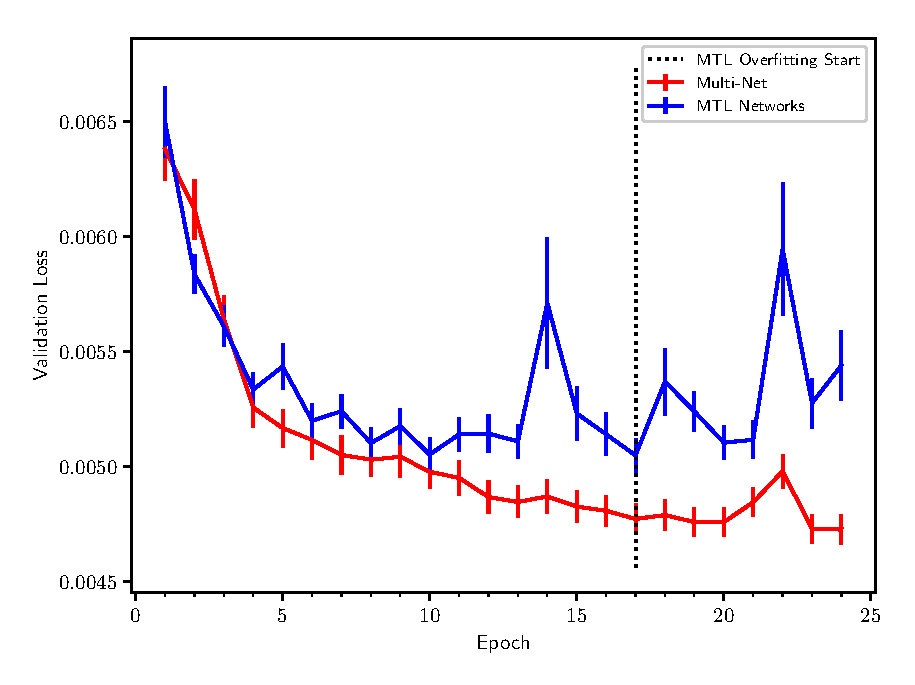
\includegraphics[width=\linewidth]{paper/content/images/mtl}
\caption{Multi-Modal Validation of MultiNet and MTL Networks with 95\% Confidence Intervals}
\label{fig:lve}
\end{figure}
